\subsection{BÀI TẬP TRẮC NGHIỆM}
\ind{PHẦN I.} \inden{Câu trắc nghiệm nhiều phương án lựa chọn. Mỗi câu hỏi học sinh chỉ chọn một phương án.}\\
\setcounter{ex}{0}
\Opensolutionfile{ans}[ans/0H4-B3-1]
\begin{ex}
	Cho vectơ $\overrightarrow{a} \ne \overrightarrow{0}$. Xét vectơ $-3\overrightarrow{a}$, khẳng định nào sau đây là khẳng định \textbf{sai}?
	\choice
	{$-3\overrightarrow{a}$ cùng phương với $\overrightarrow{a}$}
	{\True $-3\overrightarrow{a}$ cùng hướng với $-3\overrightarrow{a}$}
	{$\bigg|-3\overrightarrow{a}\bigg|=3\bigg|\overrightarrow{a}\bigg|$}
	{$-3\overrightarrow{a}$ có giá trùng với $\overrightarrow{a}$}
	\loigiai{
	}
\end{ex}
\begin{ex}
	Cho ba điểm $A,B,M$ được xác định như hình bên. Tìm đẳng thức đúng.
	\immini{	
		\choice
		{$\overrightarrow{AM}=\dfrac{2}{3}\overrightarrow{MB}$}
		{\True $\overrightarrow{AM}=-2\overrightarrow{AB}$}
		{$\overrightarrow{AM}=2\overrightarrow{AB}$}
		{$\overrightarrow{AM}=\dfrac{3}{2}\overrightarrow{MB}$}
	}{
		\hspace{1cm}
		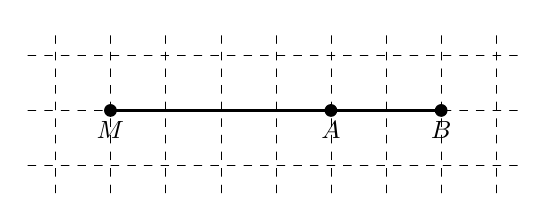
\begin{tikzpicture}[>=stealth,scale=0.7, line join=round, line cap=round]
			\draw[line width=0.07pt,dashed] (-0.5,-0.5) grid (8.5,2.5);
			\draw[fill=black] (1,1) circle(3pt) (5,1) circle(3pt) (7,1) circle(3pt);
			\draw[line width = 1.4pt] (1,1)node[below]{\small$M$}--(5,1)node[below]{\small$A$}--(7,1) node[below]{\small$B$};
	\end{tikzpicture}}
	\loigiai{
}
\end{ex}


\begin{ex}%[0H1Y3-2]
	Cho ba điểm phân biệt $A$, $B$, $C$. Nếu $\overrightarrow{AB}=-3\overrightarrow{AC}$ thì đẳng thức nào dưới đây đúng?
	\choice
	{$\overrightarrow{BC}=-2\overrightarrow{AC}$}
	{\True$\overrightarrow{BC}=4\overrightarrow{AC}$}
	{$\overrightarrow{BC}=2\overrightarrow{AC}$}
	{$\overrightarrow{BC}=-4\overrightarrow{AC}$}
	\loigiai{
		Ta có $\overrightarrow{BC}=\overrightarrow{AC}-\overrightarrow{AB}=\overrightarrow{AC}-\left(-3\overrightarrow{AC}\right)=4\overrightarrow{AC}.$}
\end{ex}

\begin{ex}%[0H1B3-2]
	Cho $I$ là trung điểm của đoạn $AB$. Chọn mệnh đề đúng trong các mệnh đề sau?
	\choice
	{$IA+IB=0$}
	{\True $\overrightarrow{IA}+\overrightarrow{IB}=\overrightarrow{0}$}
	{$\overrightarrow{AI}=-\overrightarrow{IB}$}
	{$\overrightarrow{AI}=\overrightarrow{BI}$}
	\loigiai{
		Do $I$ là trung điểm của đoạn thẳng $AB$ nên hai vectơ $\overrightarrow{IA}, \overrightarrow{IB}$ đối nhau. Vậy $\overrightarrow{IA}+\overrightarrow{IB}=\overrightarrow{0}$.}
\end{ex}


\begin{ex}%[0H1B3-4]
	\immini[thm]{Cho hình bình hành $ABCD$. Trong các mệnh đề sau, mệnh đề nào đúng?
		\choice
		{$\overrightarrow{AC}=\overrightarrow{AB}-\overrightarrow{AD}$}
		{$\overrightarrow{AC}=\overrightarrow{AB}+2\overrightarrow{AD}$}
		{\True $\overrightarrow{AC}=\overrightarrow{AB}+\overrightarrow{AD}$}
		{$\overrightarrow{AC}=2\overrightarrow{AB}+\overrightarrow{AD}$}
	}{
		\begin{tikzpicture}[scale=0.7, line join=round, line cap=round]
			\tkzDefPoints{0/0/A,4/0/B,5/2/C}
			\tkzDefPointBy[translation=from B to C](A)\tkzGetPoint{D}
			\tkzDrawSegments(A,B B,C C,D D,A)
			\tkzDrawPoints[size=2,fill=black](A,B,C,D)
			\tkzLabelPoints[below,font=\footnotesize](A, B)
			\tkzLabelPoints[above,font=\footnotesize](C,D)
	\end{tikzpicture}}
	\loigiai{
		Áp dụng quy tắc hình bình hành ta có $\overrightarrow{AC}=\overrightarrow{AB}+\overrightarrow{AD}$.
	}
\end{ex}

\begin{ex}%[0H1Y3-2]
	\immini[thm]{Cho $G$ là trọng tâm tam giác $ABC$, gọi $I$ là trung điểm của $BC$. Đẳng thức nào sau đây \textbf{đúng}?
		\choice
		{\True$\overrightarrow{GB}+\overrightarrow{GC}=2\overrightarrow{GI}$}
		{$\overrightarrow{GB}+\overrightarrow{GC}=\overrightarrow{GA}$}
		{$\overrightarrow{GA}=2\overrightarrow{GI}$}
		{$\overrightarrow{IG}=-\dfrac{1}{3}\overrightarrow{IA}$}
	}{
		\begin{tikzpicture}[scale=0.7, line join=round, line cap=round]
			\tkzDefPoints{0/0/B,4/0/C,1/2/A}
			\coordinate (I) at ($(C)!0.5!(B)$);
			\tkzDrawSegments(A,B B,C C,A A,I)
			\tkzDrawPoints[size=2,fill=black](A,B,C,I)
			\tkzLabelPoints[below,font=\footnotesize](C, B,I)
			\tkzLabelPoints[above,font=\footnotesize](A)
	\end{tikzpicture}}
	\loigiai{
		Áp dụng quy tắc trung điểm: vì $I$ là trung điểm của $BC$ nên $\overrightarrow{GB}+\overrightarrow{GC}=2\overrightarrow{GI}$.}
\end{ex}

\begin{ex}%[0H1B3-2]
	Cho $\triangle ABC$ có $G$ là trọng tâm và $M$ là trung điểm của $BC$. Mệnh đề nào sau đây là đúng?
	\choice
	{\True $\overrightarrow{GB}+\overrightarrow{GC}=2\overrightarrow{GM}$}
	{$\overrightarrow{AM}=\dfrac{2}{3}\overrightarrow{AG}$}
	{$\overrightarrow{GB}+\overrightarrow{GC}=2\overrightarrow{GA}$}
	{$\overrightarrow{AB}+\overrightarrow{AC}=2\overrightarrow{AG}$}
	\loigiai{
		\immini{
			Ta có
			\begin{itemize}
				\item $\overrightarrow{GB}+\overrightarrow{GC}=2\overrightarrow{GM}=-\overrightarrow{GA}$.
				\item $\overrightarrow{AB}+\overrightarrow{AC}=2\overrightarrow{AM}=3\overrightarrow{AG}$.
				\item $\overrightarrow{AM}=\dfrac{3}{2}\overrightarrow{AG}$.
			\end{itemize}
		}{
			\begin{tikzpicture}[scale=1, line join=round, line cap=round]
				\tkzDefPoints{0/0/B,5/0/C,2/3/A}
				\tkzCentroid(A,B,C)\tkzGetPoint{G}
				\coordinate (M) at ($(B)!0.5!(C)$);
				\tkzDrawPoints[size=2,fill=black](A,B,C,M,G)
				\tkzDrawSegments(A,B B,C C,A A,M G,B G,C)
				\tkzMarkSegments[mark=x](B,M M,C)
				\tkzLabelPoints[above](A)
				\tkzLabelPoints[below left](B)
				\tkzLabelPoints[below right](C)
				\tkzLabelPoints[below](M)
				\tkzLabelPoints[above right](G)
			\end{tikzpicture}
	}}
\end{ex}

\begin{ex}%[0H1B3-3]
	Cho tam giác $ABC$. Gọi $G$ là trọng tâm của tam giác $ABC$ và $M$ là trung điểm của $BC$. Tìm mệnh đề đúng?
	\choice
	{$\overrightarrow{AB}+\overrightarrow{AC}=\overrightarrow{AM}$}
	{$\overrightarrow{GB}+\overrightarrow{GC}=2\overrightarrow{GA}$}
	{\True $\overrightarrow{GB}+\overrightarrow{GC}=2\overrightarrow{GM}$}
	{$\overrightarrow{GB}+\overrightarrow{GC}=\overrightarrow{GA}$}
	\loigiai{
		Ta có $\overrightarrow{GB}+\overrightarrow{GC}=2\overrightarrow{GM}$.}
\end{ex}

\begin{ex}%[0H1Y3-4]
	Cho tam giác $ABC$ có $M$ là trung điểm của $BC$. Trong các mệnh đề sau, mệnh đề nào \textbf{sai}?
	\choice
	{$2\overrightarrow{AM}=2\overrightarrow{AB}+\overrightarrow{BC}$}
	{$2\overrightarrow{AM}=\overrightarrow{AB}+\overrightarrow{AC}$}
	{\True $2\overrightarrow{AM}=2\overrightarrow{AC}+\overrightarrow{BC}$}
	{$2\overrightarrow{AM}=2\overrightarrow{AC}-\overrightarrow{BC}$}
	\loigiai{
		Giả sử phương án \textbf{D} đúng. Ta có $2\overrightarrow{AM}=2\overrightarrow{AC}+\overrightarrow{BC}$, suy ra $2\overrightarrow{CM}=\overrightarrow{BC}$. Hơn nữa $2\overrightarrow{MC}=\overrightarrow{BC}$. Từ đó suy ra $\overrightarrow{CM}=\overrightarrow{0}$. Mâu thuẫn với giả thiết $M$ là trung điểm của $BC$.}
\end{ex}

\begin{ex}%[Hung Tran Nguyen Khai]%[1081-1100 Nguyễn Tiến Thùy]%[0H1K3-1]%
	Cho hình bình hành $ABCD$, $M$ là trung điểm $AB$, $DM$ cắt $AC$ tại $I$. Mệnh đề nào sau đây là đúng?
	\choice
	{$ \vec{AI}=\dfrac{3}{4}\vec{AC} $}
	{$ \vec{AI}=\dfrac{1}{4}\vec{AC} $}
	{\True $ \vec{AI}=\dfrac{1}{3}\vec{AC} $}
	{$ \vec{AI}=\dfrac{2}{3}\vec{AC}$}
	\loigiai{
		\immini{
			Đường thẳng $AB\parallel CD$ cắt hai cạnh $CI$, $DI$ của tam giác $CDI$ lần lượt tại $A$, $M$. Áp dụng định lí Thales ta có
			\begin{center} $\dfrac{AM}{CD}=\dfrac{AI}{IC}=\dfrac{MI}{ID}=\dfrac{1}{2}$.
			\end{center}
			Từ đó ta có $\dfrac{AI}{AI+IC}=\dfrac{1}{1+2}=\dfrac{1}{3}$.\\
			Vậy $\vec{AI}=\dfrac{1}{3}\vec{AC}$.
		}{
			\begin{tikzpicture}[scale=1, line join=round, line cap=round]
				\tkzDefPoints{0/0/A,4/0/B,5/2.5/C,1/2.5/D}
				\coordinate (M) at ($(A)!0.5!(B)$);
				\tkzInterLL(A,C)(D,M)\tkzGetPoint{I}
				\tkzDrawSegments(A,B B,C C,D D,A A,C D,M)
				\tkzDrawPoints[size=5,fill=black](A,B,C,D,M,I)
				\tkzLabelPoints[below left](A)
				\tkzLabelPoints[](B)
				\tkzLabelPoints[left,yshift=3pt](I)
				\tkzLabelPoints[below](M)
				\tkzLabelPoints[above right](C)
				\tkzLabelPoints[above left](D)
			\end{tikzpicture}
	}}
\end{ex}

\begin{ex}%[0H1B3-6]
	Cho $\overrightarrow{u} \ne \overrightarrow{0}$ và điểm $A$ cố định. Tập hợp tất cả điểm $M$ trong mặt phẳng thoả mãn $\overrightarrow{u}$ và $\overrightarrow{AM}$ cùng phương là
	\choice
	{một điểm cố định}
	{một đường tròn}
	{tập hợp rỗng}
	{\True một đường thẳng}
	\loigiai{
		Ta có $\overrightarrow{u}$ và $\overrightarrow{AM}$ cùng phương suy ra giá của $\overrightarrow{u}$ song song hoặc trùng với giá của $\overrightarrow{AM}$ hay tập hợp điểm $M$ trong mặt phẳng là một đường thẳng qua $A$ song song hoặc trùng với giá của $\overrightarrow{u}$.
	}
\end{ex}

\begin{ex}%[0H1B3-2]
	Cho tam giác $ABC$. Gọi $I$ là trung điểm của $AB$. Tìm điểm $M$ thỏa mãn hệ thức $\overrightarrow{MA}+\overrightarrow{MB}+2\overrightarrow{MC}=\overrightarrow{0}$.
	\choice
	{$M$ là trung điểm của $BC$}
	{$M$ là trung điểm của $IA$}
	{$M$ là điểm trên cạnh $IC$ sao cho $IM=2MC$}
	{\True $M$ là trung điểm của $IC$}
	\loigiai{
		Do $I$ là trung điểm $AB$ nên $\overrightarrow{MA}+\overrightarrow{MB}=2\overrightarrow{MI}$. Suy ra
		\begin{eqnarray*}
			& &\overrightarrow{MA}+\overrightarrow{MB}+2\overrightarrow{MC}=\overrightarrow{0}\\
			& \Leftrightarrow & 2\overrightarrow{MI}+2\overrightarrow{MC}=\overrightarrow{0}\\
			& \Leftrightarrow & \overrightarrow{MI}+\overrightarrow{MC}=\overrightarrow{0}
		\end{eqnarray*}
		Vậy $M$ là trung điểm $IC$.
	}
\end{ex}




\begin{ex}%[0H1B3-4]
	Cho tam giác $ABC$ với $G$ là trọng tâm. Đặt $\overrightarrow{CA}=\overrightarrow{a}$, $\overrightarrow{CB}=\overrightarrow{b}$. Khi đó, $\overrightarrow{AG}$ được biểu diễn theo hai vectơ $\overrightarrow{a},\overrightarrow{b}$ là
	\choice
	{$\overrightarrow{AG}=\dfrac{\overrightarrow{2a}+\overrightarrow{b}}{3}$}
	{\True $\overrightarrow{AG}=\dfrac{\overrightarrow{-2a}+\overrightarrow{b}}{3}$}
	{$\overrightarrow{AG}=\dfrac{\overrightarrow{a}-2\overrightarrow{b}}{3}$}
	{$\overrightarrow{AG}=\dfrac{\overrightarrow{2a}-\overrightarrow{b}}{3}$}
	\loigiai{
		Theo quy tắc trọng tâm ta có
		\begin{eqnarray*}
			&&\overrightarrow{GA}+\overrightarrow{GB}+\overrightarrow{GC}=\overrightarrow{0}\\
			&\Leftrightarrow& \overrightarrow{AG}=\overrightarrow{GB}+\overrightarrow{GC}=\overrightarrow{GA}+\overrightarrow{AB}+\overrightarrow{GA}+\overrightarrow{AC}\\
			&\Leftrightarrow&3\overrightarrow{AG}=\overrightarrow{AB}+\overrightarrow{AC}=\overrightarrow{AC}+\overrightarrow{CB}+\overrightarrow{AC}=\overrightarrow{CB}-2\overrightarrow{CA}\\
			&\Leftrightarrow&\overrightarrow{AG}=\dfrac{\overrightarrow{CB}-2\overrightarrow{CA}}{3}=\dfrac{\overrightarrow{b}-2\overrightarrow{a}}{3}.
	\end{eqnarray*}}
\end{ex}

\begin{ex}%[0H1K3-5]
	Cho tam giác $ABC$ và điểm $D$ thoả mãn $\overrightarrow{AD}=m\overrightarrow{AB}+n\overrightarrow{AC}$. Điều kiện cần và đủ để điểm $D$ thuộc đường thẳng $BC$ là
	\choice
	{$m-n=1$}
	{$mn=1$}
	{\True $m+n=1$}
	{$m=n=\dfrac{1}{2}$}
	\loigiai{
		Từ giả thiết ta có
		\begin{align*}
			&\overrightarrow{BD}-\overrightarrow{BA}=-m\overrightarrow{BA}+n\left(\overrightarrow{BC}-\overrightarrow{BA}\right)\\
			&\Leftrightarrow \overrightarrow{BD}= (1-m-n)\overrightarrow{BA}+n\overrightarrow{BC}.
		\end{align*}
		Điểm $D$ thuộc đường thẳng $BC$ khi và chỉ khi tồn tại số $k$ sao cho $\overrightarrow{BD}=k\overrightarrow{BC}$\\
		Thay vào đẳng thức ở trên ta được:
		\begin{align*}
			&k\overrightarrow{BC}= (1-m-n)\overrightarrow{BA}+n\overrightarrow{BC}\\
			&\Leftrightarrow (k-n)\overrightarrow{BC}= (1-m-n)\overrightarrow{BA}.
		\end{align*}
		Từ đó suy ra $k-n=1-m-n=0$. Vậy $m+n=1$.
	}
\end{ex}

\begin{ex}%[0H1Y3-1]
	Cho tam giác $ABC$ vuông cân tại $A$, $AB=a$. Tính độ dài vectơ $\overrightarrow{AB}+4\overrightarrow{AC}$.
	\choice
	{$17a$}
	{\True $\sqrt{17}a$}
	{$5a$}
	{$\sqrt{20}a$}
	\loigiai{
		\immini{Dựng các điểm $D,E$ sao cho $\overrightarrow{AD}=4\overrightarrow{AC}$ và tứ giác $ABED$ là hình bình hành.
			Khi đó \\ $\left|\overrightarrow{AB}+4\overrightarrow{AC}\right| = \left|\overrightarrow{AB} +\overrightarrow{AD}\right| = \left|\overrightarrow{AE}\right| = \sqrt{a^2+(4a)^2} = a\sqrt{17}$.
		}
		{
			\begin{tikzpicture}[scale=0.8,font=\footnotesize,line join=round,
				line cap=round,>=stealth]
				\tkzInit[xmin=-0.5,ymin=-0.5,xmax=8.5,ymax=3.0]\tkzClip
				%\pgfresetboundingbox
				\tkzDefPoints{0/0/A,2/0/C}
				\tkzDefPointBy[rotation = center A angle 90](C)\tkzGetPoint{B}
				\tkzDefPointBy[homothety = center A ratio 4](C)\tkzGetPoint{D}
				\tkzDefPointBy[translation = from A to B](D)\tkzGetPoint{E}
				\tkzDrawSegments[->](A,B A,D A,E A,C)
				\tkzDrawSegments(B,C)
				\tkzDrawSegments[dashed](E,B E,D)
				\tkzDrawPoints(A,B,C,D,E)
				\tkzLabelPoints[below](A,D,C)
				\tkzLabelPoints[above](B,E)
				\tkzMarkRightAngles(C,A,B)
			\end{tikzpicture}
		}
	}
\end{ex}

\begin{ex}%[0H1G3-1]
	Cho tam giác vuông cân $OAB$ với $OA=OB=a$. Độ dài của $\overrightarrow{u}=\dfrac{21}{4}\overrightarrow{OA}+\dfrac{5}{2}\overrightarrow{OB}$ là
	\choice
	{$\dfrac{\sqrt{140}}{4}a $}
	{\True $\dfrac{\sqrt{541}}{4}a$}
	{$\dfrac{\sqrt{520}}{4}a $}
	{$ \dfrac{\sqrt{321}}{4}a $}
	\loigiai{
		Dựng hình chữ nhật $OMNP$ sao cho $\overrightarrow{OM}=\dfrac{21}{4}\overrightarrow{OA},\,\overrightarrow{OP}=\dfrac{5}{2}\overrightarrow{OB}$. Ta có $OM=\dfrac{21}{4}a,\,ON=\dfrac{5}{2}a$.\\
		Áp dụng quy tắc hình bình hành, ta có $\overrightarrow{ON}=\overrightarrow{OM}+\overrightarrow{OP}\Rightarrow ON=\sqrt{OM^2+OP^2}=\dfrac{\sqrt{541}}{4}a.$}
\end{ex}


\Closesolutionfile{ans}

\ind{PHẦN II.} \inden{Câu trắc nghiệm đúng sai. Trong mỗi ý a), b), c), d) ở mỗi câu, học sinh chọn đúng hoặc sai.}\\
\Opensolutionfile{ans}[ans/0H4-B3-2]
\begin{ex}%[0H1B3-1]
	Cho $\overrightarrow{a}$ và $\overrightarrow{b}$ là các vectơ khác $\overrightarrow{0}$ sao cho $\overrightarrow{a}=\dfrac{2018}{2019}\overrightarrow{b}$. Xét tính đúng sai của các khẳng định sau:
	\choiceTF
	{\True$\overrightarrow{a}$ và $\overrightarrow{b}$ cùng hướng}
	{$a=\dfrac{2018}{2019}b$}
	{\True $\overrightarrow{b}=\dfrac{2019}{2018}\overrightarrow{a}$}
	{ $\left|\overrightarrow{a}\right|>\left|\overrightarrow{b}\right|$}
	\loigiai{
	}
\end{ex}

\begin{ex}%[0H5H3-9]
	Máy bay $A$ đang bay về hướng đông bắc với tốc độ $600$ km/h. Cùng lúc đó, máy bay $B$ đang bay về hướng tây nam với tốc độ $800$ km/h (như hình vẽ).
	\begin{center}
		\begin{tikzpicture}[scale=1,>=stealth, font=\footnotesize, line join=round, line cap=round,declare function={a=2;h=1;db=15;tn=-135;}]
			%------------máy bay
			\tikzset{maybay/.pic={
					%Đuôi máy bay
					\def\D{  (-2,-.45)--(-2.36,.24)--(-2.2,.3)--(-1.35,-.25)--cycle
						;}
					\draw \D;
					\fill[brown!40!] \D;
					
					%Quạt máy bay
					\def\Q{  (.15,-.1)
						..controls +(-140:0.1) and +(140:0.1) .. (.2,-.35)--(.8,-.17)--(.7,.07)--cycle
						
						;}
					\draw \Q;
					\draw[xshift=.5cm] \Q;
					\fill[brown!40!,xshift=.5cm] \Q;
					%---------elip2
					\draw[rotate=-70,xshift=-.23cm,yshift=1.27cm] (.7,-.1) ellipse (.12cm and .07cm);
					
					%Thân máy bay
					\def\T{  (-2.1,-.5)
						..controls +(40:0) and +(-170:0.7) .. (2,.74)
						..controls +(-40:0) and +(170:0.3) .. (2.55,.7)
						..controls +(-150:0) and +(30:.65) .. (2.1,.3)
						..controls +(-150:0) and +(-18:1.25) .. (-2.1,-.6)
						..controls +(90:0) and +(-90:0) .. (-2.1,-.51)
						-- (-2.5,-.52)--cycle;
					}
					\draw \T;
					\fill[brown!70!] \T;
					%Cánh máy bay
					\def\C{  (.5,.05)
						..controls +(170:0) and +(-10:0) .. (-1.48,.12)
						..controls +(-80:0) and +(170:0.02) .. (-1.65,.3)
						..controls +(180:0) and +(0:0) .. (-1.77,.3)
						..controls +(-80:0) and +(110:0) .. (-1.64,.12)
						..controls +(-35:0) and +(145:0) .. (-.2,-.17)
						--cycle
						;}
					\draw \C;
					\fill[brown!40!] \C;
					%Quạt sau
					\fill[brown!40!] \Q;
					%----elip 1
					\draw[rotate=-70,xshift=-.4cm,yshift=.8cm] (.7,-.1) ellipse (.12cm and .07cm);
					%Ô cửa
					\draw (2.18,0.73)--(2.5,0.7)--(2.14,0.58)--cycle;
					\fill[brown!40!](2.18,0.73)--(2.51,0.71)--(2.14,0.57)--cycle;
			}}
			\path
			(2,1) coordinate (A)
			(A)+(0.5,0.4)coordinate (M)
			(M)+(db+17:0.9)coordinate (N)
			(A)+(2,-h) coordinate (B)
			(B)+(-0.4,-0.1)coordinate (P)
			(P)+(tn-17:1.2)coordinate (Q)
			(A)+(-2,-1)coordinate (O)
			(O)+(-0.8,0)coordinate (x')
			(O)+(0.8,0)coordinate (x)
			(O)+(0,-0.8)coordinate (y')
			(O)+(0,0.8)coordinate (y)
			;
			
			\path(A) pic[shift={(80:.15)},scale=.2,rotate=db,yscale=1]{maybay};
			\path(B) pic[shift={(80:.15)},scale=.2,rotate=tn,yscale=-1]{maybay};
			\draw[-stealth](M)--(N);
			\draw[-stealth](P)--(Q);
			\path ($(M)!0.5!(N)$)node[shift={(90:.25)},scale=1]{$\vec{a}$};
			\path ($(P)!0.5!(Q)$)node[shift={(-90:.25)},scale=1]{$\vec{b}$};
			\foreach \p/\g in{A/-60,B/-60}
			\path(\p)node[shift={(\g:.2)},scale=1]{$\p$};
			%%%%La bàn
			\draw[-stealth,line width=1.5pt](O)--(x')node[shift={(-180:.4)},scale=1]{Tây};
			\draw[-stealth,line width=1.5pt](O)--(x)node[shift={(0:.5)},scale=1]{Đông};
			\draw[-stealth,line width=1.5pt](O)--(y')node[shift={(-90:.2)},scale=1]{Nam};
			\draw[-stealth,line width=1.5pt](O)--(y)node[shift={(90:.2)},scale=1]{Bắc};
			
			\draw[fill=white,line width=1.5pt](O)circle(0.15);
			\shade[shading=ball](O)circle(.05);
			
		\end{tikzpicture}
	\end{center}
	Xét tính đúng sai của các khẳng định sau:
	\choiceTF
	{\True Vectơ vận tốc $\vec{b}$ của máy bay $B$ ngược hướng với vectơ vận tốc $\vec{a}$ của máy bay $A$}
	{$\vec{a}=600$ km/h, $\vec{b}=800$ km/h}
	{$\vec{b}=\dfrac{4}{3}\vec{a}$}
	{\True $\big|\vec{a}+\vec{b}\big|=200$ (km/h)}
	\loigiai{
	\begin{itemchoice}
		\itemch Đúng. Hướng đông bắc và hướng tây nam là hai hướng hoàn toàn ngược nhau.
		\itemch Sai. Vận tốc là đại lượng vectơ, còn tốc độ là độ lớn của vectơ vận tốc. Do đó, cách viết đúng phải là $|\vec{a}| = 600$ km/h và $|\vec{b}| = 800$ km/h. Việc cho một vectơ bằng một số vô hướng là sai bản chất toán học.
		\itemch Sai. Hai vectơ $\vec{a}$ và $\vec{b}$ ngược hướng, tỉ số độ lớn là $\dfrac{|\vec{b}|}{|\vec{a}|} = \dfrac{800}{600} = \dfrac{4}{3}$. Do đó, biểu diễn đúng phải có dấu trừ: $\vec{b} = -\dfrac{4}{3}\vec{a}$. Khẳng định đã cho thiếu dấu trừ.
		\itemch Đúng. Do $\vec{a}$ và $\vec{b}$ là hai vectơ ngược hướng nên độ dài của vectơ tổng bằng trị tuyệt đối của hiệu hai độ lớn:
		$$ |\vec{a} + \vec{b}| = \big| |\vec{a}| - |\vec{b}| \big| = |600 - 800| = |-200| = 200 \text{ (km/h)}. $$
	\end{itemchoice}
}
\end{ex}

\begin{ex}%[0H1B3-1]
	Cho $\triangle ABC$ có $G$ là trọng tâm. $M$ là một điểm bất kì. Xét tính đúng sai của các khẳng định sau:
	\choiceTF
	{$ \overrightarrow{GB}+\overrightarrow{GC}=2\overrightarrow{GA} $}
	{\True $ 3\overrightarrow{AG}=\overrightarrow{AB}+\overrightarrow{AC} $}
	{\True $ \overrightarrow{GA}+\overrightarrow{GB}+\overrightarrow{GC}=\overrightarrow{0} $}
	{\True $ \overrightarrow{MA}+\overrightarrow{MB}+\overrightarrow{MC}=3\overrightarrow{MG},~\forall M $}
	\loigiai{
	\begin{itemchoice}
		\itemch Sai. Gọi $I$ là trung điểm của $BC$, theo quy tắc trung điểm ta có $\overrightarrow{GB} + \overrightarrow{GC} = 2\overrightarrow{GI}$. Mà $G$ là trọng tâm nên $\overrightarrow{GA} = -2\overrightarrow{GI}$. Do đó $\overrightarrow{GB} + \overrightarrow{GC} = -\overrightarrow{GA}$.
		\itemch Đúng. Gọi $I$ là trung điểm của $BC$, theo quy tắc trung điểm $\overrightarrow{AB} + \overrightarrow{AC} = 2\overrightarrow{AI}$. Vì $G$ là trọng tâm nên $AI = \dfrac{3}{2}AG \Rightarrow \overrightarrow{AI} = \dfrac{3}{2}\overrightarrow{AG}$. Thay vào ta được: $\overrightarrow{AB} + \overrightarrow{AC} = 2 \cdot \dfrac{3}{2}\overrightarrow{AG} = 3\overrightarrow{AG}$.
		\itemch Đúng. Đây là tính chất cơ bản của trọng tâm tam giác.
		\itemch Đúng. Đây là tính chất mở rộng của trọng tâm tam giác đối với một điểm $M$ bất kì trong mặt phẳng.
	\end{itemchoice}
}
\end{ex}

\begin{ex}%[0H1B3-4]
	Cho hình bình hành $ABCD$ có $O$ là giao điểm của $AC$ và $BD$, $G$ là trọng tâm tam giác $ABC$. Xét tính đúng sai của các khẳng định sau:
	\choiceTF
	{$\overrightarrow{OA}+\overrightarrow{OB}=\overrightarrow{BA}$}
	{\True$\overrightarrow{AO}=\dfrac{1}{2}\left(\overrightarrow{AB}+\overrightarrow{AD}\right)$}
	{$\overrightarrow{OA}+\overrightarrow{OB}=\overrightarrow{OC}+\overrightarrow{OD}$}
	{$\vec{AG}=\dfrac{1}{6}\overrightarrow{AB}+\dfrac{5}{6}\overrightarrow{AD}$}
	\loigiai{
	\begin{itemchoice}
		\itemch Sai. Gọi $M$ là trung điểm của $AB$, ta có $\overrightarrow{OA} + \overrightarrow{OB} = 2\overrightarrow{OM}$. Hai vectơ $2\overrightarrow{OM}$ và $\overrightarrow{BA}$ không thể bằng nhau (chúng có phương vuông góc với nhau trong trường hợp hình thoi).
		\itemch Đúng. Theo quy tắc hình bình hành, $\overrightarrow{AB} + \overrightarrow{AD} = \overrightarrow{AC}$. Mà $O$ là tâm hình bình hành nên $O$ là trung điểm $AC \Rightarrow \overrightarrow{AC} = 2\overrightarrow{AO}$. Vậy $\overrightarrow{AO} = \dfrac{1}{2}(\overrightarrow{AB} + \overrightarrow{AD})$.
		\itemch Sai. Vì $O$ là trung điểm của $AC$ và $BD$ nên $\overrightarrow{OA} = -\overrightarrow{OC}$ và $\overrightarrow{OB} = -\overrightarrow{OD}$. Do đó $\overrightarrow{OA} + \overrightarrow{OB} = -\overrightarrow{OC} - \overrightarrow{OD} = -(\overrightarrow{OC} + \overrightarrow{OD})$. Khẳng định hai vế bằng nhau là vô lý.
		\itemch Sai. Vì $G$ là trọng tâm tam giác $ABC$ nên $\overrightarrow{AG} = \dfrac{1}{3}(\overrightarrow{AB} + \overrightarrow{AC})$. Áp dụng quy tắc hình bình hành $\overrightarrow{AC} = \overrightarrow{AB} + \overrightarrow{AD}$, thay vào ta được:
		$$ \overrightarrow{AG} = \dfrac{1}{3}(\overrightarrow{AB} + \overrightarrow{AB} + \overrightarrow{AD}) = \dfrac{2}{3}\overrightarrow{AB} + \dfrac{1}{3}\overrightarrow{AD}. $$
		Hệ số của khẳng định đã cho ($\dfrac{1}{6}$ và $\dfrac{5}{6}$) là hoàn toàn sai.
	\end{itemchoice}
}
\end{ex}

\Closesolutionfile{ans}

\ind{PHẦN III.} \inden{Câu trắc nghiệm trả lời ngắn.}\\
\Opensolutionfile{ans}[ans/0H4-B3-3]


\begin{ex}%[GHK1, THPT Lương Thế Vinh CS1 - Hà Nội, 2019]%[Dương BùiĐức, 10-EX-1-19]%[0H1K3-1]%
	Cho tam giác vuông cân $ABC$ với $AB=AC=\sqrt{5}$. Tính $\big|2\vec{AB}+\vec{AC}\big|$.\\
	\shortans[oly]{$5$}
		\loigiai{
		\immini{
			Dựng điểm $ E $ sao cho $ \vec{AE}=2\vec{AB} $ và điểm $ D $ sao cho $ AEDC $ là hình bình hành, khi đó $ \vec{AD}=2\vec{AB}+\vec{AC} $. Ta có
			\[
			AE=2\sqrt{5}\Rightarrow AD=\sqrt{AE^{2}+AC^{2}}=5.
			\]
		}{
			\begin{tikzpicture}[line join=round, line cap=round,font=\small]
				\pgfmathsetmacro\h{1}
				\pgfmathsetmacro\goc{45}
				\pgfmathsetmacro\x{3*\h}
				\pgfmathsetmacro\y{2*\h}
				\pgfmathsetmacro\xmin{-0.5*\x}
				\pgfmathsetmacro\xmax{1.5*\x}
				\pgfmathsetmacro\ymin{-1.8*\y}
				\pgfmathsetmacro\ymax{1.2*\y}
				\clip(\xmin-0.01,\ymin-0.01)rectangle(\xmax+0.01,\ymax+0.01);
				\tkzDefPoint(0,0){B}
				\tkzDefShiftPoint[B](0:\x){b}
				\tkzDefShiftPoint[B](\goc:\y){A}
				\tkzDefLine[orthogonal=through A](A,B)\tkzGetPoint{a}
				\tkzInterLL(A,a)(B,b)\tkzGetPoint{C}
				\tkzDefPointsBy[homothety = center A ratio 2](B){E}
				\coordinate (D) at ($(C)+(E)-(A)$);
				\tkzDrawPoints[fill=black](A,B,C,E,D)
				\draw (A)--(E)--(D)--(C)--cycle;
				\draw (B)--(C);
				\tkzDrawSegment[->,dashed](A,D)
				\tkzLabelPoints[below](B,C,E,D)
				\tkzLabelPoints[above](A)
				\tkzMarkRightAngles(C,A,B)
			\end{tikzpicture}
		}
	}
\end{ex}

\begin{ex}%[Tex hóa BTN 10]%[Người soạn:Ngụy Như Thái -PB:Nguyễn Tài Tuệ]%[0H1B3-1]%
	Cho tam giác $ABC$ đều có cạnh $AB=5$, $H$ là trung điểm của $BC$. Tính $\left|\vec{CA}-\vec{HC}\right|$ (kết quả làm tròn đến 1 chữ số thập phân).\\
	\shortans[oly]{$6,6$}
	\loigiai{
		\begin{center}
			\begin{tikzpicture}[>=stealth,line join=round,line cap=round,font=\footnotesize,scale=1]
				\tkzDefPoints{0/0/B, 3/5/A}
				\tkzDefEquilateral(A,B)\tkzGetPoint{C}
				\coordinate (H) at ($(B)!.5!(C)$);
				\coordinate (E) at ($(A)!.5!(H)$);
				\draw (A)node[above]{$A$}--(B)node[below left]{$B$}--(C)node[below right]{$C$}--(A)--(E)node[above left]{$E$}--(H)node[below]{$H$}--(C)--(E);
				\tkzMarkRightAngle[size=0.3,fill=gray!20](E,H,C)
				\tkzDrawPoints[size=7,fill=black](A,B,C,H,E)
			\end{tikzpicture}
		\end{center}
		Ta có: $\left|\vec{CA}-\vec{HC}\right|=\left|\vec{CA}+\vec{CH}\right|=\left|2\vec{CE}\right|=2CE$ (với $E$ là trung điểm của $AH$).\newline
		Ta lại có: $AH=\dfrac{5\sqrt 3}{2}$ ($\Delta ABC$ đều, $AH$ là đường cao).\newline
		Trong tam giác $HEC$ vuông tại $H$, có:\newline
		$EC=\sqrt{C{H^2}+H{E^2}}=\sqrt{2.5^2+\left(\dfrac{5\sqrt 3}{4}\right)^2}=\dfrac{5\sqrt 7}{4}$ $\Rightarrow\left|\vec{CA}-\vec{HC}\right|=2CE=\dfrac{5\sqrt 7}{2} \approx6,6$.}
\end{ex}

\begin{ex}%[0H5V3-5]
	Cho hình bình hành $ABCD$. Gọi $M$ là trung điểm của cạnh $BC$. Biết rằng $\vec{AM}=x\vec{AB}+y\vec{AD}$. Tính $2x+y$ (làm tròn đến chữ số thập phân thứ hai).\\
	\shortans[oly]{$2{,}50$}
	\loigiai{
		\immini{Ta có
			\begin{eqnarray*}
				\vec{AM}&=&\dfrac{1}{2}\left(\vec{AB}+\vec{AC}\right)\\
				&=&\dfrac{1}{2}\left(\vec{AB}+\vec{AB}+\vec{AD}\right)\\
				&=&\vec{AB}+\dfrac{1}{2}\vec{AD}.
			\end{eqnarray*}
		}
		{
			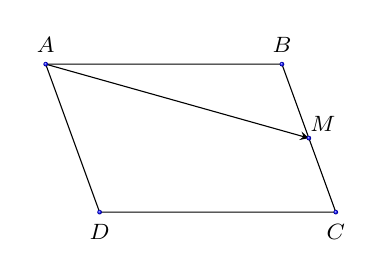
\begin{tikzpicture}[scale=1,>=stealth, font=\footnotesize, line join=round, line cap=round,declare function={h=2;}]
				\path
				(0,0) coordinate (A)
				(3,0) coordinate (B)
				(B)+(-70:h) coordinate (C)
				(A)+(-70:h) coordinate (D)
				(barycentric cs:C=1,B=1)coordinate(M)
				
				;
				\draw (A)--(B)--(C)--(D)--(A);
				\draw[-stealth](A)--(M);
				\foreach \p/\g in{A/90,B/90,C/-90,D/-90,M/45}
				\shade[shading=ball](\p)circle(.03)node[shift={(\g:.25)},scale=1]{$\p$};
			\end{tikzpicture}
		}
		\noindent Vậy $2x+y=2\cdot1+\dfrac{1}{2}=\dfrac{5}{2}\approx 2{,}50$.
	}
\end{ex}


\begin{ex}
	Cho tam giác $ABC$ và ba điểm $M$, $N$, $P$ xác định bởi 
	\begin{listEX}[3]
		\item [] $\vec{MB}+2\vec{MC}=\vec{0}$,
		\item [] $3\vec{NC}=\vec{NA}$,
		\item [] $\vec{PA}=k\vec{PB}$, với $k \ne 1$.
	\end{listEX}
Tìm $k$ để ba điểm $M$, $N$, $P$ thẳng hàng.\\
	\shortans[oly]{$-1,5$}
	\loigiai{
		Có $\vec{NM}=\dfrac{1}{3}\vec{NB}+\dfrac{2}{3}\vec{NC}$ và $\vec{NP}=\dfrac{1}{1-k}\vec{NA}-\dfrac{k}{1-k}\vec{NB}=-\dfrac{k}{1-k}\vec{NB}+\dfrac{3}{1-k}\vec{NC}$.\\
		Do đó $M$, $N$, $P$ thẳng hàng khi
		$$\dfrac{-\dfrac{k}{1-k}}{\dfrac{1}{k}}=\dfrac{\dfrac{3}{1-k}}{\dfrac{2}{3}} \Rightarrow k=-\dfrac{3}{2}.$$
	}
\end{ex}

\begin{ex}%[0H1K3-7]
	Cho $\triangle ABC$ có trọng tâm $G$, $H$ là chân đường cao kẻ từ $A$ sao cho $\overrightarrow{BH}=\dfrac{1}{3}\overrightarrow{HC}$. Điểm $M$ di động trên $BC$ sao cho $\overrightarrow{BM}=x\overrightarrow{BC}$. Tìm $x$ sao cho $\left|\overrightarrow{MA}+\overrightarrow{GC}\right|$ nhỏ nhất (kết quả làm trong 2 chữ số thập phân).\\
	\shortans[oly]{$0{,}83$}
	\loigiai{
		\immini{$\left|\overrightarrow{MA}+\overrightarrow{GC}\right|=\left|\overrightarrow{MA}+\overrightarrow{AG}+\overrightarrow{BG}\right|=\left|\overrightarrow{MG}+\overrightarrow{BG}\right|=2\left|\overrightarrow{GI}\right|$, với $I$ là trung điểm $BM$. \\
			Vậy $\left|\overrightarrow{MA}+\overrightarrow{GC}\right|$ nhỏ nhất khi $GI$ nhỏ nhất hay $I$ là hình chiếu của $G$ trên $BC$. \\
			Gọi $F$ là trung điểm $BC$. \\
			Ta có $\overrightarrow{BH}=\dfrac{1}{3}\overrightarrow{HC}$ suy ra: $H$ là trung điểm của $BF$ (1). \\
			Vì $G$ là trọng tâm nên $HI=\dfrac{2}{3}FH$ (2). \\
			Từ $(1)$ và $(2)$ suy ra: $BI=\dfrac{5}{6}BF \Leftrightarrow BM=\dfrac{5}{6}BC \Rightarrow \overrightarrow{BM}=\dfrac{5}{6}\overrightarrow{BC}$. \\
			Vậy $x=\dfrac{5}{6}$.}
		{\begin{tikzpicture}[scale=0.9, line join=round, line cap=round]
				\tkzDefPoints{1.2/3.5/A,0/0/B,5/0/C}
				\tkzCentroid(A,C,B)\tkzGetPoint{G}
				\tkzDefPointBy[projection=onto C--B](A)\tkzGetPoint{a}
				\coordinate (F) at ($(C)!0.5!(B)$);
				\coordinate (E) at ($(A)!1/2!(C)$);
				\coordinate (M) at ($(B)!0.8!(C)$);
				\tkzInterLL(A,F)(B,E)\tkzGetPoint{G}
				\tkzDefPointBy[projection=onto C--B](G)\tkzGetPoint{i}
				\tkzInterLL(A,a)(B,C)\tkzGetPoint{H}
				\tkzInterLL(G,i)(B,C)\tkzGetPoint{I}
				\tkzDrawPolygon(A,C,B)
				\tkzDrawSegments(A,F A,H G,I)
				\tkzDrawPoints[fill=black](A,C,B,F,G,H,I,M)
				\tkzLabelPoints[below](C,F,B,H,I,M)
				\tkzLabelPoints[above](A)
				%\tkzLabelPoints[above left](E)
				\tkzLabelPoints[above right](G)
				\tkzMarkRightAngle[size=0.2](A,H,C)
		\end{tikzpicture}}
	}
\end{ex}



\Closesolutionfile{ans}

